% -------------------------------------------------------------------------------------------------------
%-----------------------------CONSULTA DE RECURSOS HUMANOS---------------------------------
% -------------------------------------------------------------------------------------------------------

\chapter{Gestión de Recursos Humanos}
    Para poder ver la lista de recursos humanos que tiene a su cargo, primero debe seleccionar la opción \textbf{Gestionar Recursos Humanos} del menú ubicado en la parte izquierda, así podrá observar la siguiente pantalla:

        % Imagen de Consultar recursos humanos
        \begin{figure}[H]
            \centering
            \hypertarget{consultarRH}{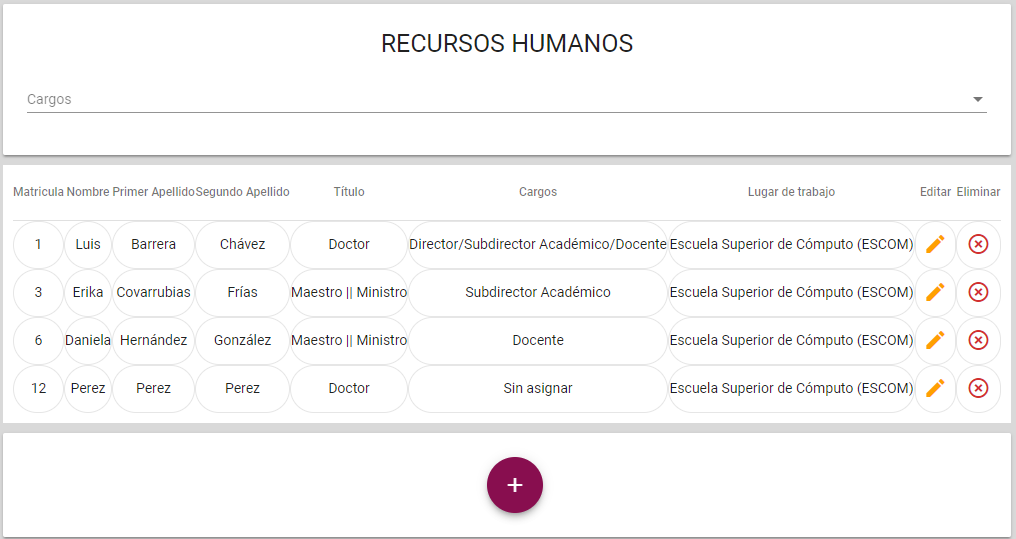
\includegraphics[width=0.7\linewidth]{images/SP1/ConsultarRH}}
            \caption{Pantalla para consultar recursos humanos}
            \label{consultarrh}
        \end{figure}

        En esa pantalla, aparecerán de forma predeterminada todos los recursos humanos que tiene a su cargo y que están registrados en el sistema hasta el momento. Tendrá a su disposición 2 funciones:
        \newpage
        \begin{enumerate}

            \item   Buscar recursos humanos según el cargo que ocupan.

                Para esto solo tendrá que seleccionar el cargo que desea consultar en el siguiente componente:

                \begin{figure}[H]
                    \centering
                    \hypertarget{cargo1}{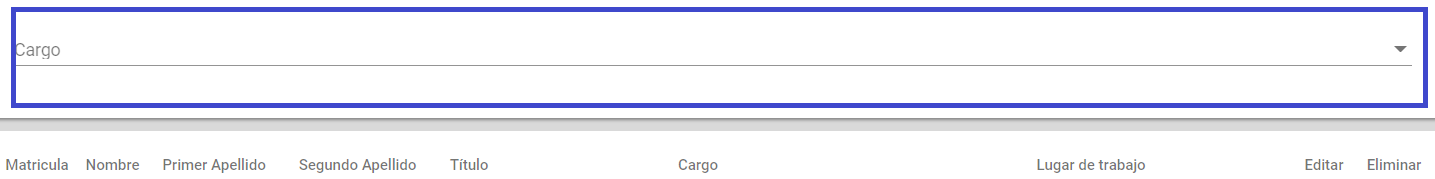
\includegraphics[width=0.7\linewidth]{images/SP1/BtnCargo1}}
                    \caption{Selección de Cargo}
                    \label{cargo1}
                \end{figure}

                 Y a continuación el sistema mostrará todos los recursos humanos que tengan el cargo seleccionado.

                    \item Eliminar recursos humanos.

                Para esta última acción, usted solo deberá dar clic en el botón con el icono de una equis en color rojo que está al lado del recurso humano que desee  eliminar.

                \begin{figure}[H]
                    \centering
                    \hypertarget{eliminar}{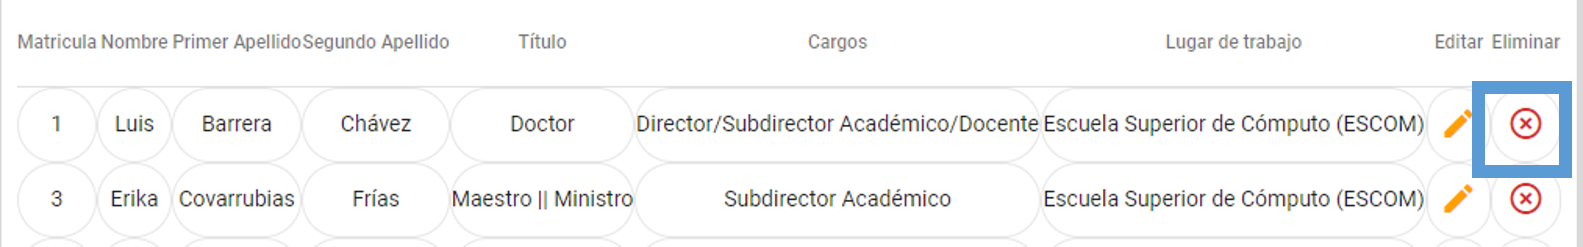
\includegraphics[width=0.7\linewidth]{images/SP1/BtnEliminar}}
                    \caption{Botón Eliminar Recursos Humanos}
                    \label{eliminar}
                \end{figure}

                Al hacer esto, el sistema desplegara el siguiente mensaje:

                %Imagen del MSG22
               \begin{figure}[H]
                    \centering
                    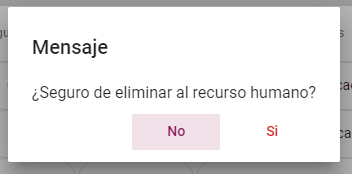
\includegraphics[width=0.4\linewidth]{images/SP1/MSG22}
                \caption{Confirmación de eliminación}
                \label{confirmarE}

                \end{figure}

                Para confirmar, usted deberá dar clic en el botón “Sí”, y en ese momento el recurso humano será removido del sistema y usted permanecerá en la pantalla \hyperlink{consultarRH}{\textit{Consultar Recursos Humanos}}.
                Para cancelar, usted deberá dar clic en botón “No”, y en ese momento el mensaje se cerrara, el recurso humano no se eliminará, y usted permanecerá en la pantalla de \hyperlink{consultarRH}{\textit{Consultar Recursos Humanos}}.



        \end{enumerate}

        También mediante botones de esta pantalla podrá acceder a las siguientes 2 funciones:

        \subsection{Editar recursos humanos}

            Para esto, usted solo deberá dar clic en el botón con el icono de un lápiz amarillo que está al lado del recurso humano que desea modificar. Al hacer esto el sistema le mostrará la pantalla   de \hyperlink{editarRH}{\textit{Editar Recurso Humano}}.

            \begin{figure}[H]
                \centering
                \hypertarget{editar}{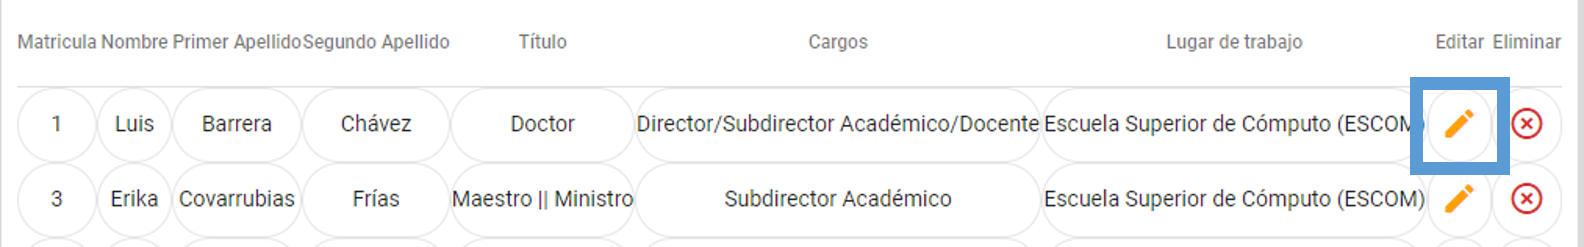
\includegraphics[width=0.7\linewidth]{images/SP1/BtnEditar}}
                \caption{Botón Editar Recursos Humanos}
                \label{editar}
            \end{figure}

            Para más detalles de editar usuarios vaya a la sección \hyperlink{editar-RH}{Edición de Recursos Humanos}.

        \subsection{Registrar recursos humanos}

            Para esto solo tendrá que dar clic en el botón “+” en la parte inferior de la pantalla. Al hacerlo, el sistema  lo redireccionará a la pantalla de \hyperlink{registrarRH}{\textit{Registrar Recurso Humano}}.

            \begin{figure}[H]
                \centering
                \hypertarget{add}{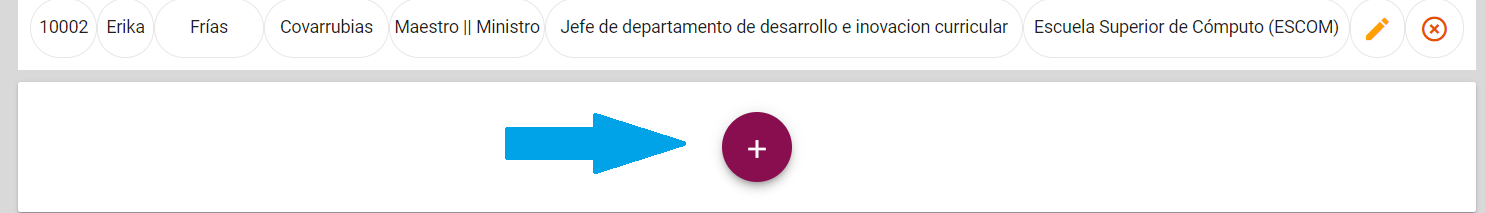
\includegraphics[width=0.7\linewidth]{images/SP1/BtnAgregar}}
                \caption{Botón Agregar Recursos Humanos}
                \label{add}
            \end{figure}

            Para más detalles de registrar recursos humanos vaya a la sección \hyperlink{registrar}{Registar recurso humano}.

        \subsection{Posibles errores}
          \begin{itemize}
                \item Si al  presionar la opción Gestionar Recursos Humanos no se carga la información de los cargos disponibles para usted se presentara el siguiente mensaje:

            % Imagen del MSG7
             \begin{figure}[H]
                \centering
                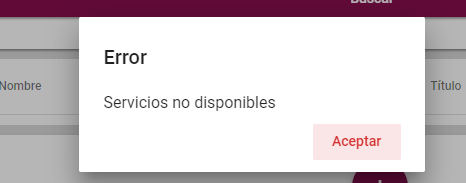
\includegraphics[width=0.4\linewidth]{images/SP1/MSGSN}
                \caption{Servicios no disponibles}
                \label{SND}

            \end{figure}

                    Al dar clic en en botón ''Aceptar'', el sistema continuara en la pantalla  \hyperlink{consultarRH}{\textit{Consultar Recursos Humanos}} y tendrá que intentarlo  mas tarde.


              \item Si al intentar eliminar un recurso humano aparece el siguiente mensaje:
              % Imagen del MSG56
                \begin{figure}[H]
                   \centering
                   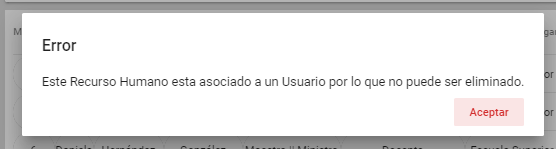
\includegraphics[width=0.4\linewidth]{images/SP1/MSG56}
                    \caption{Recurso humano asociado a un usuario no puede ser eliminado}
                   \label{mensaje56}
                \end{figure}

                Significa que ese recurso humano tiene una cuenta de usuario registrada en el sistema. Primero, debe de ir a la opción \textbf{Gestionar Usuarios} del menú ubicado en la parte izquierda y eliminar su cuenta de usuario.

                Para más detalles de eliminar un recurso humano registrado como usuario en el sistema vaya a la sección \hyperlink{consultarUs}{\textit{Consultar Usuarios}}.


           \end{itemize}

           %%% MENSAJE DE VINCULACION CON USUARIO


        % ------------------------------------------------------------------------------------
        % ----------------------------- REGISTRAR  USUARIOS ---------------------------------
        % ------------------------------------------------------------------------------------

    \newpage
        \hypertarget{registrarRH}{}
        \section{Registrar Recursos Humanos}
            Si usted  en la pantalla de \hyperlink{consultarRH}{\textit{Consultar Recursos Humanos}} dio clic en el botón ''+'', aparece la siguiente pantalla:

            \begin{figure}[H]
                \centering
                \hypertarget{registrarUs}{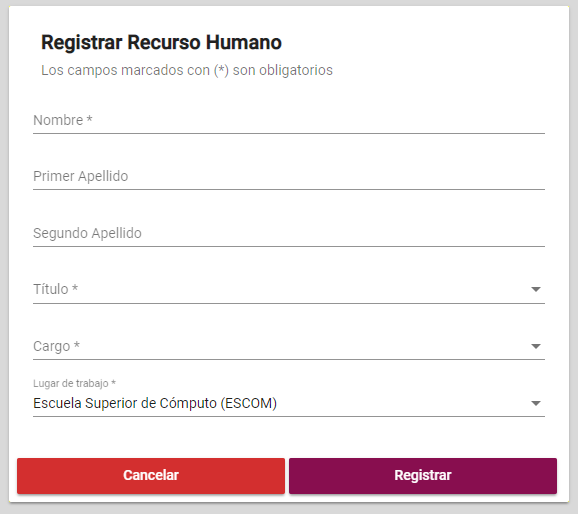
\includegraphics[width=0.7\linewidth]{images/SP1/RegistrarRH}}
                \caption{Pantalla para registar recursos humanos}
                \label{registrarrh}
            \end{figure}

            Usted tendrá que ingresar la información correspondiente del nuevo recurso humanos en el formulario. Un ejemplo del llenado seria el siguiente:

            \begin{figure}[H]
                \centering
                \hypertarget{ejreg}{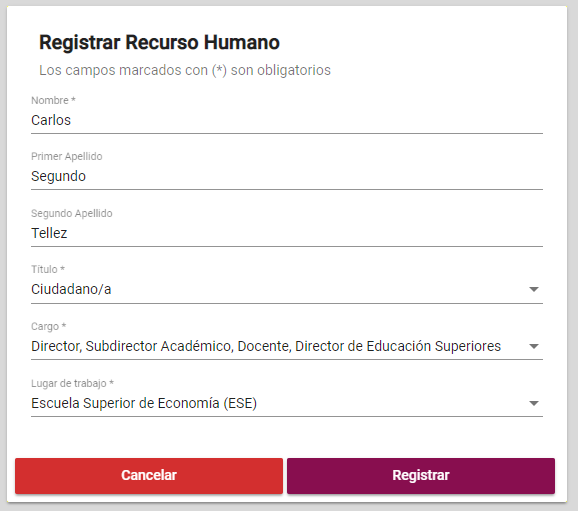
\includegraphics[width=0.7\linewidth]{images/SP1/RegistrarLleno}}
                \caption{Ejemplo de llenado para agregar un nuevo recurso humano}
                \label{ejreg}
            \end{figure}

    \newpage
            Si usted presiona el botón de “Cancelar”:

            \begin{figure}[H]
                \centering
                \hypertarget{cancel1}{
\includegraphics[width=0.7\linewidth]{images/SP1/BtnCancelar1}}
                \caption{Botón ''Cancelar''}
                \label{cancel1}
            \end{figure}

            El sistema mostrará el siguiente mensaje:

            %Imagen MSG29

             \begin{figure}[H]
                \centering
            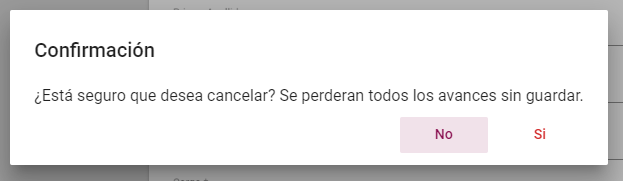
\includegraphics[width=0.4\linewidth]{images/SP1/MSG29}
                \caption{Cancelar Accion}
                \label{mensaje29}
            \end{figure}

            Para confirmar, usted tendrá que dar clic en el botón “Sí”, el recurso humano no será registrado y regresara a la pantalla de \hyperlink{consultarRH}{\textit{Consultar Recursos Humanos}}.

            Para continuar con el registro, usted tendrá que  dar clic el botón “No”, el mensaje se cerrara y usted continuara en el formulario para terminar el registro.

            Cuando usted considere que los datos son correctos y están completos, deberá de dar clic en el botón “Registrar”.

            \begin{figure}[H]
                \centering
                \hypertarget{btnreg}{
\includegraphics[width=0.7\linewidth]{images/SP1/BtnRegistrar}}
                \caption{Botón ''Registrar''}
                \label{btnreg}
            \end{figure}

            Si no se presentan errores el sistema muestra el mensaje:

            % Imagen MSG5

             \begin{figure}[H]
                \centering
            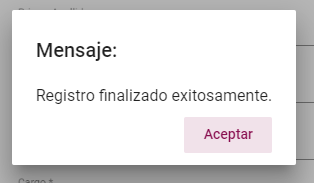
\includegraphics[width=0.4\linewidth]{images/SP1/MSG5}
                \caption{Registro exitoso}
                \label{mensaje5}

            \end{figure}

            Al dar clic en el botón “Aceptar”, el sistema mostrará la pantalla de  \hyperlink{consultarRH}{\textit{Consultar Recursos Humanos}}.

            \subsection{Posibles errores}

                \begin{itemize}
                    \item Problemas con la conexión o el sistema

                        Si al momento de acceder a la pantalla de \hyperlink{registrarRH}{\textit{Registrar Recurso Humano}} o al intentar registrar un recurso humano , aparece el siguiente mensajes:
                        %Imagen MSG7 Y MSG25

                        \begin{figure}[H]
                        \centering
                        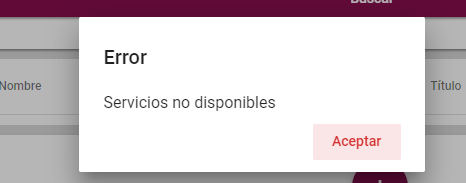
\includegraphics[width=0.4\linewidth]{images/SP1/MSGSN}
                        \caption{Servicios no disponibles}
                        \label{SND}

                      \end{figure}

                        Significa que existió un error de conexión o del sistema. Al dar clic en en botón ''Aceptar'', el sistema lo redireccionará a la pantalla de \hyperlink{consultaRH}{\textit{Consultar Recursos Humanos}}. Deberá esperar a que la página este disponible para  intentar acceder nuevamente.

                    \item Campos vacíos al momento de agregar un nuevo recurso humano

                        Si usted deja en blanco algún campo o campos del formulario, y posteriormente dio clic en el botón ''Registrar'', el sistema mostrará el siguiente mensaje debajo del campo o campos :
                        %Imagen MSG44

                         \begin{figure}[H]
                            \centering
                        
\includegraphics[width=0.4\linewidth]{images/SP1/MSG44}
                            \caption{Campos vacíos}
                        \label{mensaje44}
                       \end{figure}

                         Regresara al formulario, en donde usted deberá llenar el o los campos que dejo vacíos.

                    \item Los campos ingresados no son válidos

                        Si al momento de dar clic en el botón ''Registrar'' aparece el siguiente mensaje:
                        %Imagen MSG35
                             % Imagen del MSG35
                         \begin{figure}[H]
                            \centering
                            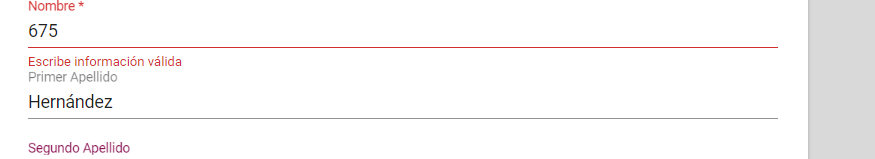
\includegraphics[width=0.4\linewidth]{images/SP1/MSG35}
                            \caption{Campos incorrectos}
                            \label{mensaje35}

                        \end{figure}

                        Significa que la composición de los datos ingresados en el formulario no es la correcta. Tenga en cuenta lo siguiente:

                        \begin{itemize}
                            \item El nombre y apellidos debe iniciar con mayúscula, puede poner más de uno por campo en caso de 2 nombres o apellidos compuestos.
                            \item Usted alteró la información de los selectores de cargo o zona de trabajo.
                            %\item La contraseña no acepta acentos, espacios o caracteres especiales.
                        \end{itemize}

                \end{itemize}

            % ------------------------------------------------------------------------------------
            % ------------------------------ EDICION DE USUARIOS ---------------------------------
            % ------------------------------------------------------------------------------------
\newpage

            \hypertarget{editar-RH}{}
            \section{Edición de Recursos Humanos}
                Si el Jefe de Innovación Educativa en la pantalla de \hyperlink{consultarRH}{\textit{Consultar Recursos Humanos}} dio clic en el botón con el icono de un lápiz amarillo de un recurso humano, aparece la siguiente pantalla:

                \begin{figure}[H]
                    \centering
                    \hypertarget{editarUs}{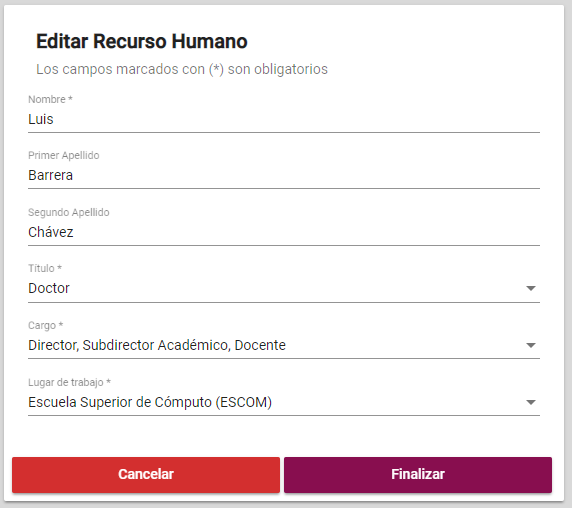
\includegraphics[width=0.6\linewidth]{images/SP1/EditarRH}}
                    \caption{Pantalla para la edición de recursos humanos}
                    \label{editarrh}
                \end{figure}

                En esta pantalla se cargarán los datos del recurso humano correspondiente por el lápiz amarillo seleccionado en la pantalla de \hyperlink{consultarRH}{\textit{Consultar Recursos Humanos}} y llenará el formulario.

                A continuación, usted podrá modificar todos los campos del recurso humano.

                Si usted presiona el botón de “Cancelar”:

                \begin{figure}[H]
                    \centering
                    \hypertarget{cancel2}{
\includegraphics[width=0.7\linewidth]{images/SP1/BtnCancelar2}}
                    \caption{Botón ''Cancelar''}
                    \label{cancel2}
                \end{figure}

                El sistema mostrará el siguiente mensaje:
                %Imagen MSG29
                  \clearpage
                 \begin{figure}[H]
                    \centering
                    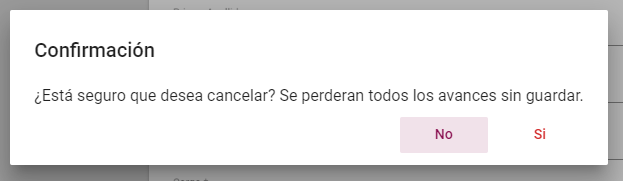
\includegraphics[width=0.4\linewidth]{images/SP1/MSG29}
                    \caption{Cancelar cambios}
                    \label{mensaje29}

                \end{figure}

                Para confirmar, usted tendrá que dar clic en el botón “Sí”, los datos del recurso humano no será modificados  y regresara a la pantalla \hyperlink{consultarRH}{\textit{Consultar Recursos Humanos}}

                Para continuar con la modificación, usted tendrá que  dar clic el botón “No”, el mensaje se cerrara y usted continuara en el formulario para terminar la modificación.

                Cuando usted considere que los datos son correctos y están completos, deberá de dar clic en el botón “Finalizar”.
                \begin{figure}[H]
                    \centering
                    \hypertarget{btnfin}{
\includegraphics[width=0.7\linewidth]{images/SP1/BtnFinalizar}}
                    \caption{Botón ''Finalizar''}
                    \label{btnfin}
                \end{figure}

                Si no se presentan errores el sistema muestra el mensaje:
                %Imagen MSG31

                 \begin{figure}[H]
                    \centering
                    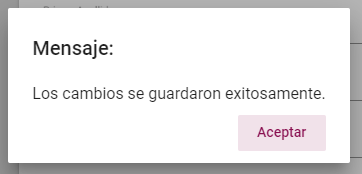
\includegraphics[width=0.4\linewidth]{images/SP1/MSG31}
                    \caption{Cambios guardados}
                    \label{mensaje31}

                \end{figure}

                Al dar clic en el botón “Aceptar”, el sistema mostrará la pantalla de \hyperlink{consultarRH}{\textit{Consultar Recursos Humanos}}.

                \subsection{Posibles errores}
                    \begin{itemize}
                        \item Problemas con la conexión o el sistema

                            Si al momento de acceder a la pantalla de \hyperlink{editarRH}{\textit{Editar Recurso Humano}} o al intentar modificar un recurso humano, aparece el siguiente mensaje:
                            \clearpage
                            \begin{figure}[H]
                                \centering
                                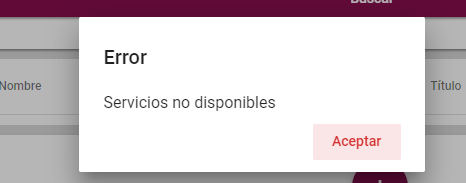
\includegraphics[width=0.4\linewidth]{images/SP1/MSGSN}
                                \caption{Servicios no disponibles}

                            \end{figure}


                            Significa que existió un error de conexión o del sistema. Al dar clic en en botón ''Aceptar'', el sistema lo redireccionará  a la pantalla de \hyperlink{consultarRH}{\textit{Consultar Recursos Humanos}}. Deberá esperar a que la página este disponible para intentar acceder nuevamente.

                        \item Campos vacíos al momento de modificar al usuario

                            Si usted deja en blanco algún campo o campos del formulario, y posteriormente dio clic en el botón ''Finalizar'', el sistema mostrará el siguiente mensaje debajo del campo o campos:
                           %Imagen MSG3X

                          \begin{figure}[H]
                            \centering
                            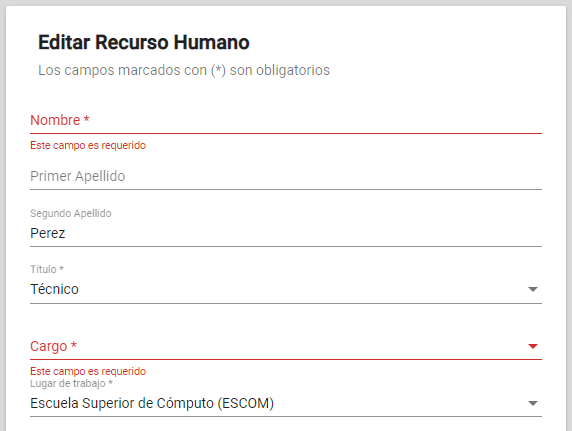
\includegraphics[width=0.4\linewidth]{images/SP1/MSG44-1}
                            \caption{Campos vacíos}
                            \label{mensaje44}

                         \end{figure}

                           Regresara  al formulario, en donde usted deberá llenar el o los campos que dejo vacíos.

                        %\item El correo ingresado ya existe

                        %Si al momento de dar clic en el botón ''Finalizar'' aparece el siguiente mensaje:
                        %Imagen MSG36

                        %\begin{figure}[H]
                            %\centering
                            %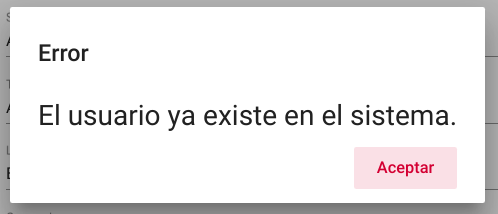
\includegraphics[width=0.4\linewidth]{images/SP1/MSG36}
                            %\caption{El usuario ya existe}
                            %\label{mensaje36}

                        %\end{figure}

                        %Significa que el Usuario ya se encuentra registrado en el sistema, por lo que éste impide que se vuelva a agregar nuevamente. Al dar clic en botón ''Aceptar'', el mensaje se cerrará y usted regresara al formulario. Aqui usted puede hacer dos acciones: verificar que el correo sea uno no registrada previamente e intentar agregar al Usuario nuevamente, o abandonar la pantalla de \hyperlink{registrarUs}{\textit{Registrar Usuarios}} e ir a otras partes del sistema.

                        \item Los campos ingresados no son válidos

                            Si al momento de dar clic en el botón ''Finalizar'' aparece el siguiente mensaje:
                            \clearpage
                                \begin{figure}[H]
                            \centering
                            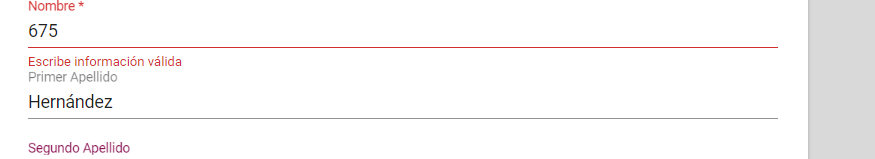
\includegraphics[width=0.4\linewidth]{images/SP1/MSG35}
                            \caption{Campos incorrectos}
                            \label{mensaje35}

                         \end{figure}


                            Significa que la composición de los datos ingresados en el formulario no es la correcta. Tenga en cuenta lo siguiente:

                            \begin{itemize}
                                \item El nombre y apellidos debe iniciar con mayúscula, puede poner más de uno por campo en caso de 2 nombres o apellidos compuestos.
                                \item Usted altero la información de los selectores de cargo o zona de trabajo.
                            \end{itemize}



                    \end{itemize}